\documentclass{beamer}
\usepackage[utf8]{inputenc}
\usepackage[]{hyperref}
\usepackage{booktabs}
\usetheme[pageofpages=of,bullet=square,
	titleline=true,
	alternativetitlepage=true,
	titlepagelogo=images/pie-no.jpg]{Torino}

\author{Statistical Reasoning\\and Quantitative Methods}
\title{Variables}
\institute{François Briatte \& Ivaylo Petev}
\date{Session 3}

%% pasted from session 2, needs to be done

%%%

\include{settings}

\begin{document}
		
	\begin{frame}[t,plain]
		\titlepage
	\end{frame}
	
	\begin{frame}[t]{Outline}
	
	A \red{variable} is something that varies over $k > 1$ states. Quantitative data is stored as variables of different \red{types}. Each type corresponds to a \red{scale of measurement} and obeys a particular numeric \red{coding}.\vspace{1em}
	
	Before we go further, a word on how the class will work from now on.
	
		\begin{columns}[T]
		\column{.35\textwidth}
			\tableofcontents[hideallsubsections]
		\column{.6\textwidth}
			\begin{center}
				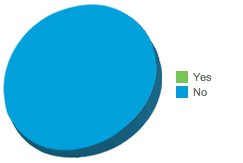
\includegraphics[scale=.5]{images/pie-no.jpg}\\[.5em]
				$k=1$ (constant)
			\end{center}		
		\end{columns}
	\end{frame}

% routines, variable types, recoding
% three routines; --> agenda file
% class routine: open stata, set wd, get do-file, follow
% homework routine: review slides, review do-files, handbook and SG
% group routine: a1, a1, final (cumul.) --> projects, template

	%
	%
	%	
	\section{Routines}
	%
	%
	%

	\begin{frame}[t]{Work routines}

	This class works through three routines:

		\begin{itemize}
			\item The \textbf{class} routine includes a `slides session' and a `do-file session'.
			
			\item The \textbf{homework} routine includes readings and replication.
			
			\item The \textbf{group} routine includes two draft papers and the final paper.
			
		\end{itemize}
	
	The last routine is the only one directly considered for grading, and within it, the \textbf{final paper} itself is the primary benchmark.\\[1em]
	
	Sections 1--4 of the Stata Guide cover the course requirements, including \textbf{computer skills} (Sec.~2) and \textbf{Stata} (Sec.~3).\\[1em]
	
	URL: \url{http://f.briatte.org/teaching/quanti/\#guide}

	\end{frame}

	\subsection{Class routine}
	
	\begin{frame}[t]{Class routine}

	From Session 4 onwards, all classes include:

	\begin{itemize}
		\item \textbf{A slide session}, to review statistical theory, learn Stata commands and go over course logistics;
		\item \textbf{A practice session}, to work on an empirical example, familiarize with a set of Stata commands and build analytical skills; and
		\item \textbf{A decent break}, because we are humans.
	\end{itemize}
		
	Check the course \textbf{syllabus} or the course \textbf{website} for the topics.\\[1em]
	
	The logic of this course requires you to
	
	\begin{enumerate}
		\item attend all sessions,
		\item replicate them at home, and
		\item read all assigned material (in that order).
	\end{enumerate}

	\end{frame}

	\begin{frame}[t]{Class routine: Details}
	
	When you get to class:
	
	\begin{itemize}
		\item \textbf{Open Stata and set the working directory} to the \code{SRQM} folder, as covered in \code{week1.do} with other Stata settings.
		\item \textbf{Get the do-file for this session} from the course website. Copy and paste it to a new-do-file window, or download it.
	\end{itemize}
	
	Check the Stata Guide for computer skill requirements (Sec.~2) and further help with Stata (Sec.~3).\\[.5em]
	
	If you attend all sessions and replicate them once at home, you will get enough training before starting to work on your research project.\\[.5em]
	
	We naturally recommend that you catch up any class that you might miss, since every session introduces new content.
	\end{frame}
	
	\subsection{Homework routine}
	
	\begin{frame}[t]{Homework routine}

	Each course session should be replicated at home:
	
	\begin{itemize}
		\item \textbf{Fetch the last course email}: this is where we send most information on course logistics.

		\item \textbf{Read the Stata Guide and handbook chapters}: both readings go hand-in-hand.
		
		\item \textbf{Replicate the course session}: make sure that you have understood the last session in full.
	\end{itemize}
	
	Check the course \textbf{syllabus} or the course \textbf{website} for the readings.\\[.5em]
	
	Each week generally has one chapter from Feinstein and Thomas' \textit{Making History Count} and at least one section of the Stata Guide.\\[.5em]
	
	\end{frame}
	
	\begin{frame}[t]{Homework routine: Details}
	
		All do-files are archived online:\vspace{.5em}
							
		\url{http://f.briatte.org/teaching/quanti/}

		\begin{itemize}
			\item Download each do-file to your \code{Replication} folder, and make sure that all course datasets are stored in the \code{Datasets} folder.
			
			\item Open Stata, set your working directory to the \textbf{SRQM} folder and adjust other settings as shown in \code{week1.do}.
			
			\item To replicate, type e.g. \code{doedit "Replication/week2.do"} and run it while reading the comments.
		\end{itemize}
		
		Check the \textbf{Stata tutorials} for help with setup and commands.\\[.5em]
		
		Replicating takes 20 minutes at most if you have all files ready and are familiar enough with Stata. Practice does it all.

	\end{frame}

	\subsection{Group routine}
	
	\begin{frame}[t]{Group routine}

	You are required to work on a research project:
		
	\begin{itemize}
		\item \textbf{Form a pair}: find someone to work with on a common theme.

		\item \textbf{Play around}: open the course datasets and inspect their content.
		
		\item \textbf{Code it}: start writing a do-file to analyse a set of variables.
	\end{itemize}
	
	Check the \textbf{Stata Guide}, Sec.~1--4 and Sec.~13--16, for instructions.\\[.5em]

	\begin{itemize}
		\item Your \textbf{do-file} should draw from the ones that we cover in class, which is why attendance and replication count so much.	
		\item Your \textbf{paper} will use the same terminology, reasoning and concepts as those that we practice in each course session.
		\item Your \textbf{final paper and do-file} will be graded twice as drafts during the semester and once at the end.
	\end{itemize}		

	\end{frame}

\begin{frame}[t]{Additional helpers}

	To help you work on all routines:
		
	\begin{itemize}
		\item \textbf{Read the course planning}: \url{http://goo.gl/BJHkQ}

		\item \textbf{Discuss your project}: \url{http://goo.gl/brYmB}
		
		\item \textbf{Look at a template}: \url{http://goo.gl/7u8oa}
	\end{itemize}
	
	All links point to course material hosted by Google Documents, which you can comment and/or edit.\\[.5em]

	Check the \textbf{course syllabus} and \textbf{Stata Guide} for additional details, which we will also introduce gradually in class.\\[.5em]
	
	The \textbf{course slides} also contain some information on how we organized the course: make sure to save them for later reviewing.\\[.5em]
	
	\red{If completely lost, email us}---but look in the course material first.
	
	\end{frame}
	
	%
	% VARIABLES
	%
	
	\section{Variables}

	\begin{frame}[t]{Variables}
	
	The essential element of quantitative analysis is called a variable. Datasets are series of variables for a given set of units.\\[.5em]
	
	The most important properties of variables are:

		\begin{itemize}
		\item Variables have \textbf{values} such as -1, 0, 1, 27 and so on.

		\item Variables have \textbf{labels} when their values require explanation.
		
		\item Variables have \textbf{missing values}; Stata codes them as `dots' (\code{.}).

		\item Variables are \textbf{manipulable}: you can modify their values and labels.
		\end{itemize}
	
		Check the Stata Guide, Sec.~5--6, for more information on variables.\\[.5em]
		
		Make sure, in particular, that you understand \textbf{continuous} and \textbf{categorical} variable types. Basically, anything that can be understood on an \textbf{ordinal scale} is continuous for our purposes.
		
	\end{frame}
	
	% measurement
	% types
	
	\section{Recoding}

	\begin{frame}[t]{Recoding}
		
		Manipulating variables is essential to analysis for several reasons:
		
		\begin{itemize}
			\item \textbf{Missing values} should be properly encoded in `\code{.}' Stata format.
			\item \textbf{Groups} can be formed out of existing measures.
			\item \textbf{Measurements} can be simplified, combined, expanded…
		\end{itemize}

		Turn to the \code{replace} and \code{recode} commands to manipulate variables.\\[.5em]
		
		In class, pay attention to terms like `continuous data', `dummies' or `nominal variables', which all point to different variable types.\\[.5em]
		
		At home, make sure that you understand the types of the variables that you are handling, and that missing values are correctly encoded.
	\end{frame}
	
		
\end{document}